\documentclass[11pt]{article}
\usepackage[a4paper,margin=2.2cm]{geometry}
\usepackage[T1]{fontenc}
\usepackage{lmodern}
\usepackage{microtype}
\usepackage{amsmath,amssymb}
\usepackage{booktabs,tabularx}
\usepackage{graphicx}
\usepackage[table]{xcolor}
\usepackage{enumitem}
\usepackage{tikz}
\usetikzlibrary{arrows.meta,positioning,fit,calc,backgrounds}
\usepackage{caption}
\usepackage[round,sort]{natbib}
\usepackage[hidelinks]{hyperref}
\usepackage{float}

\setlist{itemsep=2pt,topsep=3pt}
\setlength{\parskip}{4pt}
\setlength{\parindent}{0pt}
\setlength{\emergencystretch}{2em}
\captionsetup{font=small,labelfont=bf}
\renewcommand{\arraystretch}{1.12}

\definecolor{catc}{HTML}{2A78D6}
\definecolor{couchc}{HTML}{EB6834}
\definecolor{windowc}{HTML}{8A8F98}

\newcommand{\plain}{\paragraph{In plain words.}}
\newcommand{\precise}{\paragraph{Precisely.}}
\newcommand{\why}{\paragraph{Why this way.}}

\tikzset{
  box/.style={draw=black!75,rounded corners=1pt,align=center,font=\small,inner sep=4pt,fill=white},
  tbox/.style={box,fill=black!5},
  lbox/.style={box,fill=black!10},
  arr/.style={-{Stealth[length=2mm]},thick,draw=black!70},
  darr/.style={-{Stealth[length=2mm]},thick,dashed,draw=black!60},
}

% The toy scene in map-cell units (0..14, y upward): couch, window, cat.
\newcommand{\toyscene}{%
  \fill[couchc!45] (6,2) rectangle (13,7);
  \fill[windowc!35] (9,9) rectangle (13,13);
  \fill[catc!55] (5,7) ellipse (2 and 2.6);
}

\title{\textbf{Spatial Concept Distillation, step by step}\\[3pt]
\large What happens to one image, from the dataset to the trained student}
\author{Companion to the \texttt{concept-factors} report}
\date{}

\begin{document}
\maketitle
\vspace{-1.5em}

\begin{abstract}
\noindent This document walks through SCD one step at a time. Every step has three parts. \emph{In plain words}
explains it so that a school student could follow. \emph{Precisely} gives the shapes, formulas and numbers of
the implementation. \emph{Why this way} gives the reason for the choice. The running example is MetaShift
(1,700 training images of cats and dogs, 130 concept factors). Numbers marked ``illustrative'' are made up to
show a calculation; every other number comes from the code and the runs.
\end{abstract}

\tableofcontents
\newpage

%=====================================================================
\section{The whole method in one page}
%=====================================================================

\paragraph{For a school student.} We want a computer to learn to recognise animals from photos without anyone
telling it what is in the photos. The problem: in our photos cats almost always sit on sofas and dogs almost
always run on grass. A lazy learner decides ``sofa means cat'' and fails on a cat in the garden. So we bring in
a helper who already knows many words, a big pretrained model called CLIP. Before the lessons start, the
helper goes through every photo and colours it in like a colouring book: ``these squares are cat, these are
sofa, these are window''. During the lessons the learner looks at pieces of the photos and, for every small
square of a piece, has to say which words belong there. Because the cat and the sofa sit in \emph{different}
squares, the learner must learn what a cat looks like by itself and what a sofa looks like by itself. To stop
the learner from simply memorising the answer sheet of each photo, we check its answers with a rule built from
\emph{other} photos.

\paragraph{For the supervisor.} SCD adds one loss to SimCLR. Offline, a frozen CLIP ViT-B/32 with ClearCLIP's
last block computes, for every training image, a $14\times14$ map of soft assignments to $K$ concept factors
(text directions of synonym groups found by SpLiCE). Online, every SimCLR view's crop box and flip cut the
matching part out of its image's map and resample it to $7\times7$. The $7\times7\times512$ \texttt{layer4}
output of the ResNet-18 student must predict these $K$ values at each of its 49 locations through a ridge
regression that is fitted in closed form on one half of the batch and evaluated on the other half. The
held-out squared error, weighted by $\lambda=5$ after a warm-up, is added to the SimCLR loss.

\begin{figure}[H]
\centering
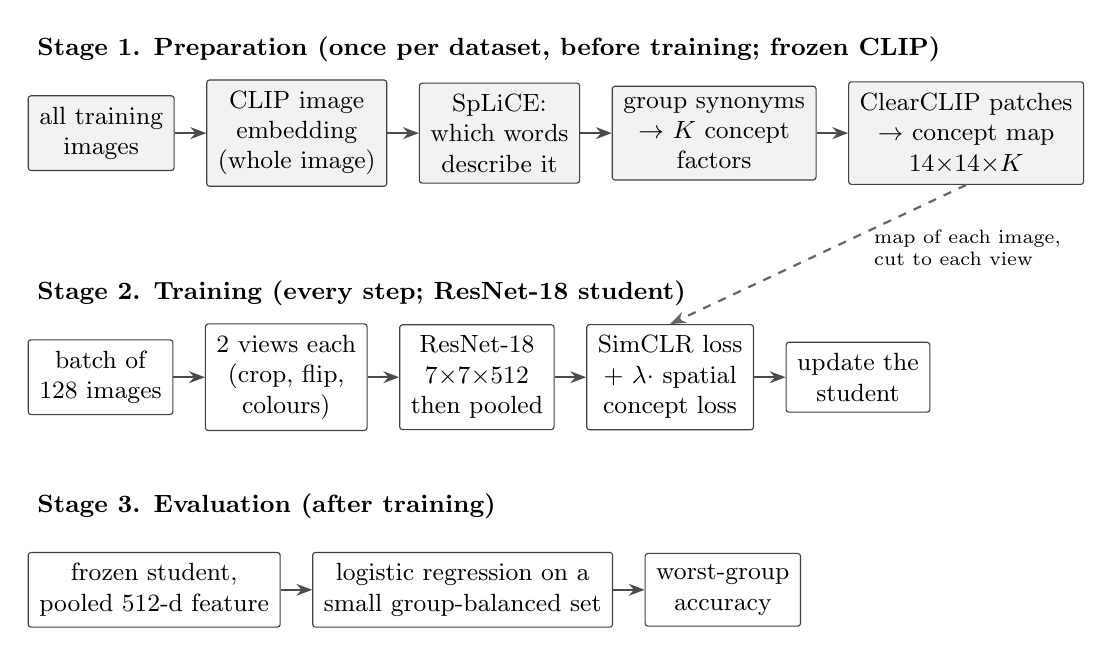
\begin{tikzpicture}[node distance=4mm and 4mm]
\node[font=\small\bfseries,anchor=west] (h1) at (0,0) {Stage 1. Preparation (once per dataset, before training; frozen CLIP)};
\node[tbox,below=3mm of h1.south west,anchor=north west] (p1) {all training\\images};
\node[tbox,right=of p1] (p2) {CLIP image\\embedding\\(whole image)};
\node[tbox,right=of p2] (p3) {SpLiCE:\\which words\\describe it};
\node[tbox,right=of p3] (p4) {group synonyms\\$\to$ $K$ concept\\factors};
\node[tbox,right=of p4] (p5) {ClearCLIP patches\\$\to$ concept map\\$14{\times}14{\times}K$};
\draw[arr] (p1)--(p2); \draw[arr] (p2)--(p3); \draw[arr] (p3)--(p4); \draw[arr] (p4)--(p5);
\node[font=\small\bfseries,anchor=west] (h2) at (0,-3.1) {Stage 2. Training (every step; ResNet-18 student)};
\node[box,below=3mm of h2.south west,anchor=north west] (t1) {batch of\\128 images};
\node[box,right=of t1] (t2) {2 views each\\(crop, flip,\\colours)};
\node[box,right=of t2] (t3) {ResNet-18\\$7{\times}7{\times}512$\\then pooled};
\node[box,right=of t3] (t4) {SimCLR loss\\+ $\lambda\cdot$ spatial\\concept loss};
\node[box,right=of t4] (t5) {update the\\student};
\draw[arr] (t1)--(t2); \draw[arr] (t2)--(t3); \draw[arr] (t3)--(t4); \draw[arr] (t4)--(t5);
\draw[darr] (p5.south) -- (t4.north);
\node[font=\scriptsize,align=left,anchor=west] at ($(p5.south)!0.45!(t4.north)+(4mm,0)$) {map of each image,\\cut to each view};
\node[font=\small\bfseries,anchor=west] (h3) at (0,-5.8) {Stage 3. Evaluation (after training)};
\node[box,below=3mm of h3.south west,anchor=north west] (e1) {frozen student,\\pooled 512-d feature};
\node[box,right=of e1] (e2) {logistic regression on a\\small group-balanced set};
\node[box,right=of e2] (e3) {worst-group\\accuracy};
\draw[arr] (e1)--(e2); \draw[arr] (e2)--(e3);
\end{tikzpicture}
\caption{The three stages. CLIP appears only in stage 1. After stage 1 only the maps are kept; after stage 2
only the ResNet-18 is kept; the maps, the projection head and every ridge fit are thrown away.}
\label{fig:overview}
\end{figure}

One correction to a natural first guess: SpLiCE runs on the embedding of the \emph{whole} image from ordinary
CLIP and its job is to choose the vocabulary. The maps come from ClearCLIP's \emph{patch} embeddings, which are
compared with the text directions of that vocabulary. SpLiCE is never applied to patches.

\begin{table}[H]
\centering
\caption{Shapes at every step for MetaShift ($N=1{,}700$ images, $K=130$ factors, batch $B=128$).}
\label{tab:shapes}
\small
\begin{tabularx}{\linewidth}{l l X}
\toprule
Step & Object & Shape \\
\midrule
1.1 & CLIP image embedding & $N\times512$ \\
1.2 & SpLiCE codes & $N\times10{,}000$, about 9 non-zero per image \\
1.3 & factor text directions $d_F$ & $K\times512$ \\
1.4 & image for the maps & $448\times448$ pixels, 9 windows of $224\times224$ \\
1.5 & ClearCLIP patch embeddings & per window $7\times7\times512$ \\
1.6 & stored concept maps & $N\times K\times14\times14$ in float16 (87 MB for MetaShift) \\
2.1 & views of a batch & $2B=256$ images of $224\times224$, each with a crop box and a flip flag \\
2.2 & student feature map (\texttt{layer4}) & $256\times512\times7\times7$ \\
2.2 & pooled feature, projection & $256\times512$, then $256\times128$ \\
2.3 & warped targets & $256\times K\times7\times7$ \\
2.4 & rows of one half & $64\cdot2\cdot49=6{,}272$ rows of 512 features and $K$ targets \\
2.4 & ridge solution $W_A$ & $512\times K$ \\
\bottomrule
\end{tabularx}
\end{table}

%=====================================================================
\section{Stage 1: preparation, once per dataset}
%=====================================================================
Stage 1 runs before training starts, on the training images only, with a frozen CLIP model (OpenCLIP ViT-B/32,
LAION-2B weights; \citealp{radford2021clip}). Nothing in it is trained and no label is used. Its output is one
file: a concept map for every training image.

\subsection{Step 1.1: one vector per image from CLIP}
\plain CLIP was trained on hundreds of millions of photos with captions, so it learned to place a photo and a
sentence that describes it close together. Give it a photo and it returns a list of 512 numbers, a ``fingerprint''
that sits close to the fingerprints of words describing the photo.

\precise The image is resized to 224 pixels and passed through CLIP's vision transformer. The class token of
the last layer, projected into the joint space, is the embedding $z_i\in\mathbb R^{512}$. Every word $k$ of a
vocabulary has a text embedding $t_k\in\mathbb R^{512}$ from CLIP's text encoder.

\why CLIP knows thousands of visual concepts from external data. It is the only source of ``names'' in the
method; the student never sees CLIP itself.

\subsection{Step 1.2: SpLiCE turns the vector into a few words}
\plain The 512 numbers are hard to read. SpLiCE rewrites the fingerprint as a short recipe: ``0.41 cat + 0.30
sofa + 0.12 blanket + \ldots'', using as few words as possible. About nine words are enough per image.

\precise With a fixed mean $\mu$ and the dictionary $D$ of text directions (10,000 LAION words for MetaShift),
SpLiCE solves \citep{bhalla2024splice}
\begin{equation}
u_i=\frac{z_i-\mu}{\lVert z_i-\mu\rVert},\qquad
c_i=\arg\min_{c\ge0}\ \lVert u_i-D^\top c\rVert_2^2+0.25\,\lVert c\rVert_1 .
\end{equation}
$c_i$ has one entry per word and about nine of them are non-zero.

\why We need to know \emph{which} concepts occur in this dataset and how often, without labels. Running SpLiCE
over all 1,700 images gives exactly that list. The rest of the method only uses this list; the per-image recipe
$c_i$ is used for counting frequencies and for the grouping in the next step.

\subsection{Step 1.3: group synonyms into concept factors}
\plain The dictionary has \emph{cat}, \emph{kitten} and \emph{kitty} as separate words. For our purpose they are one
thing. We merge words that mean the same into one ``concept factor''. A factor is a small bag of synonyms with one
common direction.

\precise Keep words active on 0.2\% to 95\% of the images. Two words are similar when the cosine of their raw
text embeddings is high; the pair is vetoed when the images' responses $u_i^\top d_k$ to the two words correlate
below 0.5. Average-linkage clustering cut at similarity 0.85 forms the groups. A factor $F$ gets the text direction
\begin{equation}
d_F=\operatorname{norm}\Big(\tfrac{1}{|F|}\textstyle\sum_{k\in F}\operatorname{norm}(t_k)\Big)
\end{equation}
and factors active on 2\% to 90\% of the images are kept: $K=130$ on MetaShift, 242 on Waterbirds, 147 on
Spur-CIFAR10. Examples: \{kitty, kitten, cat\}, \{canine, dog\}, \{couch, sofa\}.

\why Synonyms would otherwise compete with each other in every square of the map (step 1.6) and split the mass
of one thing over several names. The thresholds and the reason why the text cosine works and co-activation fails
are in Section~4.4 of the main report.

\subsection{Step 1.4: why plain CLIP is not enough for maps}
\plain We do not only want to know \emph{that} the photo contains a cat; we want to know \emph{where}. CLIP's vision
transformer cuts the image into small squares (patches) and keeps one vector per square. One would hope that the
vector of a square on the cat says ``cat''. In ordinary CLIP it does not: in the very last layer every square
``listens'' to the same few squares that collect the summary of the whole picture, so every square ends up
repeating the summary. Asking a square on the sofa what it shows gives ``cat, sofa, room'', the same answer as
every other square.

\precise CLIP is trained to align only the class token with text; nothing asks individual patch tokens to match
text. In the last block the query--key attention of every patch concentrates on the same few tokens
\citep{zhou2022maskclip,wang2024sclip}; large ViTs store global information in a few high-norm tokens
\citep{darcet2024registers}; the residual branch then adds this global signal to every patch. ClearCLIP
\citep{lan2024clearclip} changes only the last block: (i) query--query attention in place of query--key, so a patch
attends to patches that look like itself; (ii) no residual connection and (iii) no feed-forward branch. With $X$
the normalized tokens entering the last block,
\begin{equation}
P=\operatorname{norm}\Big(\operatorname{LN}\big(\operatorname{softmax}(QQ^\top/\sqrt{d_h})\,V W_O\big)W_{\text{proj}}\Big),
\qquad Q=XW_Q,\ V=XW_V,
\end{equation}
gives one unit-length vector $p(u)\in\mathbb R^{512}$ per patch $u$ in the same space as the text directions $d_F$.

\why ClearCLIP needs no training and no labels, so the restriction of the thesis holds. MaskCLIP and SCLIP follow
the same idea; ClearCLIP reports the cleanest maps of the three. The code is \texttt{patch\_embeddings} in
\texttt{cospro/pipeline/concept\_maps.py}.

\subsection{Step 1.5: reading the image through windows}
\plain ViT-B/32 cuts a 224-pixel image into a $7\times7$ grid of squares that are 32 pixels wide. That is coarse: a
cat's head and the cushion next to it fall into one square. So we enlarge the photo to 448 pixels and look at it
through nine overlapping 224-pixel windows, like reading a large map through a magnifying glass moved in steps of
half its width. Each window gives its own $7\times7$ answers and where windows overlap we average them.

\begin{figure}[H]
\centering
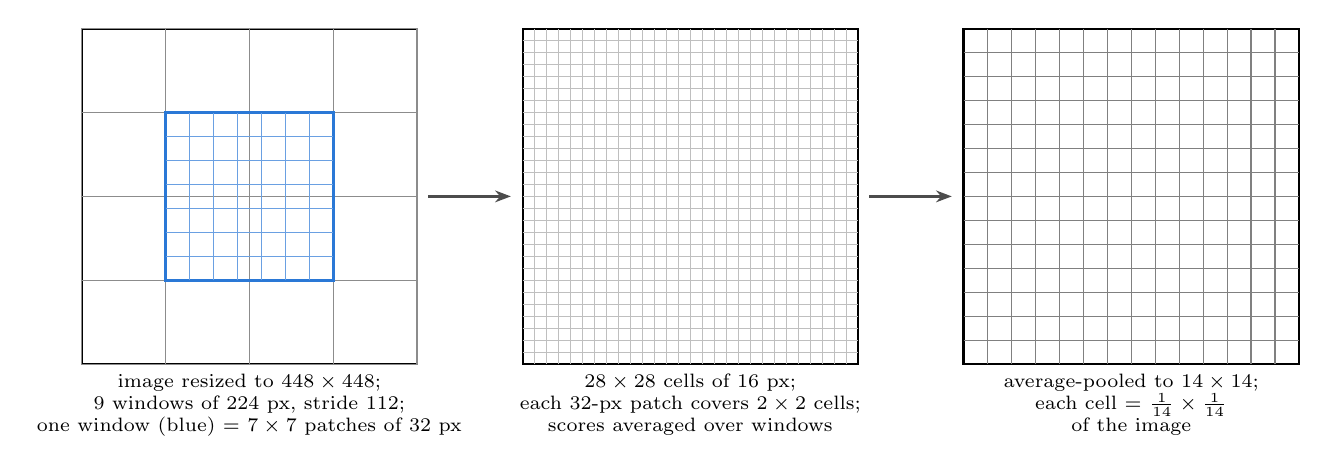
\begin{tikzpicture}
\begin{scope}[scale=0.0095]
\draw[thick] (0,0) rectangle (448,448);
\foreach \x in {0,112,224} {
  \draw[black!45,thin] (\x,0) rectangle ++(224,224);
  \draw[black!45,thin] (\x,112) rectangle ++(224,224);
  \draw[black!45,thin] (\x,224) rectangle ++(224,224);
}
\draw[very thick,catc] (112,112) rectangle ++(224,224);
\foreach \i in {1,...,6} {
  \draw[catc!70,thin] (112+\i*32,112) -- ++(0,224);
  \draw[catc!70,thin] (112,112+\i*32) -- ++(224,0);
}
\node[font=\scriptsize,align=center,below] at (224,0) {image resized to $448\times448$;\\9 windows of 224 px, stride 112;\\one window (blue) = $7\times7$ patches of 32 px};
\end{scope}
\begin{scope}[xshift=5.6cm,scale=0.0095]
\draw[thick] (0,0) rectangle (448,448);
\foreach \i in {1,...,27} { \draw[black!25,very thin] (\i*16,0) -- ++(0,448); \draw[black!25,very thin] (0,\i*16) -- ++(448,0); }
\node[font=\scriptsize,align=center,below] at (224,0) {$28\times28$ cells of 16 px;\\each 32-px patch covers $2\times2$ cells;\\scores averaged over windows};
\end{scope}
\begin{scope}[xshift=11.2cm,scale=0.0095]
\draw[thick] (0,0) rectangle (448,448);
\foreach \i in {1,...,13} { \draw[black!50,thin] (\i*32,0) -- ++(0,448); \draw[black!50,thin] (0,\i*32) -- ++(448,0); }
\node[font=\scriptsize,align=center,below] at (224,0) {average-pooled to $14\times14$;\\each cell = $\tfrac1{14}\times\tfrac1{14}$\\of the image};
\end{scope}
\draw[arr] (4.4,2.13) -- (5.45,2.13);
\draw[arr] (10.0,2.13) -- (11.05,2.13);
\end{tikzpicture}
\caption{From windows to the $14\times14$ grid. The windows start at pixels 0, 112 and 224 in each direction,
so a cell is covered by one, two or four windows.}
\label{fig:windows}
\end{figure}

\precise The image is resized (both sides, bicubic) to $448\times448$. Windows start at offsets $\{0,112,224\}$ in
each direction: $3\times3=9$ windows. Each window passes through ClearCLIP and gives $7\times7$ patch vectors.
The cosine of every patch with every factor direction, $s_F(u)=p(u)^\top d_F$, is spread onto a grid of 16-pixel
cells ($448/16=28$), averaged where windows overlap and average-pooled to $14\times14$ (\texttt{assemble\_windows}).

\why Each window stays at 224 pixels, the resolution CLIP was trained on, while the effective grid becomes 16
pixels. The stride of 112 makes every window boundary fall on a whole cell. SCLIP and ClearCLIP evaluate dense
predictions with the same sliding-window scheme \citep{wang2024sclip,lan2024clearclip}.

\subsection{Step 1.6: from scores to a concept map}
\plain For every one of the $14\times14=196$ squares we now have 130 scores: how much the square looks like
``cat'', like ``sofa'', like ``window'' and so on. We turn the scores of each square into shares that add up to
one, so that each square says ``I am 80\% cat, 15\% blanket, 5\% the rest''. Picture a colouring book in which
every square is coloured with the word that fits it best (Figure~\ref{fig:examples}).

\precise At every cell $u$ of image $i$,
\begin{equation}
M_{iF}(u)=\frac{\exp\big(s_{iF}(u)/T\big)}{\sum_{G=1}^{K}\exp\big(s_{iG}(u)/T\big)},\qquad T=0.01 .
\end{equation}
The map $M_i\in[0,1]^{K\times14\times14}$ is stored in float16. When training loads the maps, every factor is
standardized over all images and cells, $\tilde M_{iF}(u)=(M_{iF}(u)-m_F)/s_F$, so every factor has mean 0 and
variance 1.

\textit{Illustrative example.} A cell on the cat has cosines 0.27 with \emph{cat}, 0.25 with \emph{blanket} and 0.21
with \emph{sofa}. Divided by $T=0.01$ these become 27, 25 and 21; after the softmax the cell is about 88\% cat,
12\% blanket and 0.2\% sofa. With $T=1$ the three would be almost equal (34\%, 33\%, 32\%).

\why $T=0.01$ is CLIP's own scale: CLIP multiplies its cosines by a learned logit scale of 100 before its
softmax \citep{radford2021clip}. Cosines of a patch with different words differ by a few hundredths, so this scale
is what makes one word win per cell. Standardization stops frequent factors (blanket, lawn) from dominating the
squared error in step 2.4. Why $14\times14$ and not $28\times28$ or $7\times7$: step 2.3 cuts a crop out of this
map; the smallest SimCLR crop spans about $6\times6$ cells of a $14\times14$ map, enough to fill the student's
$7\times7$ grid and the stored maps stay small (87 MB for MetaShift, 455 MB for Waterbirds).

\begin{figure}[H]
\centering
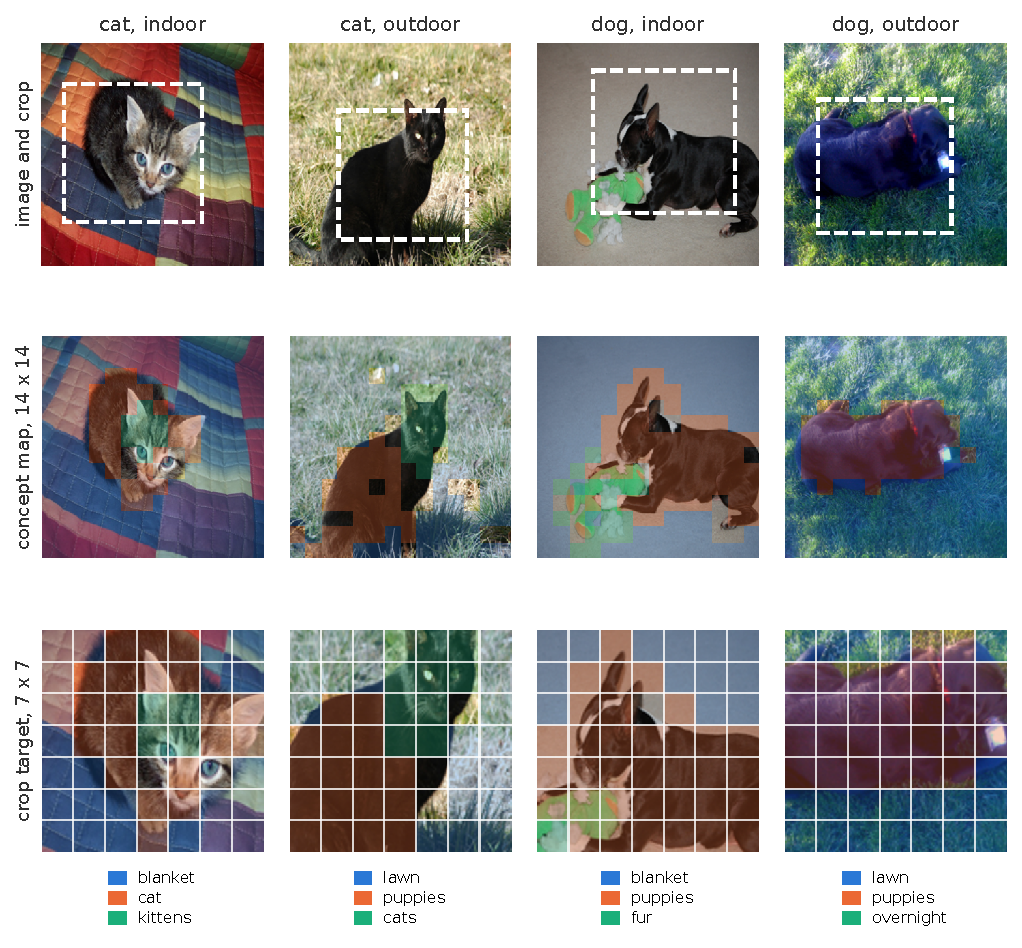
\includegraphics[width=0.85\linewidth]{figures/spatial_map_examples.pdf}
\caption{Real MetaShift maps. Top: image with one SimCLR crop (dashed). Middle: the winning factor of each of the
$14\times14$ cells. Bottom: the $7\times7$ targets that this crop receives (step 2.3). The teacher makes mistakes:
part of the black cat in the second image is labelled ``puppies''.}
\label{fig:examples}
\end{figure}

\paragraph{Output of stage 1.} One tensor of shape $N\times K\times14\times14$: for every training image and every
square of it, the share of each concept factor. Building it takes about 40 seconds on one GPU for MetaShift
(\texttt{scripts/build\_concept\_maps.sbatch}). From here on CLIP is never used again.

%=====================================================================
\section{Stage 2: one training step}
%=====================================================================
Stage 2 is ordinary SimCLR training of a ResNet-18 from random weights for 500 epochs, with one extra loss. One
epoch passes over all 1,700 images in batches of 128. Here is what happens in one step.

\subsection{Step 2.1: two views of every image}
\plain We take 128 photos. From each photo we make two ``versions'' by random edits: cut out a random piece and
blow it up to full size (crop), maybe mirror it left to right (flip), change brightness and colours, sometimes
make it grey. The two versions of one photo look different but show the same thing.

\precise The SSL transform of every view applies, in this order:
\begin{itemize}[leftmargin=*]
\item \textbf{Crop} (\texttt{RandomResizedCrop}): choose a rectangle covering 20\% to 100\% of the image area with
aspect ratio between 3:4 and 4:3, at a random position; resize it to $224\times224$.
\item \textbf{Flip} (\texttt{RandomHorizontalFlip}): mirror left--right with probability 0.5.
\item \textbf{Colour}: colour jitter (brightness, contrast, saturation 0.4, hue 0.1) with probability 0.8;
greyscale with probability 0.2.
\end{itemize}
The transform \emph{records} each view's crop box as fractions of the image (top, left, height, width) and its
flip flag (\texttt{cospro/data/transforms.py}). The batch thus holds $2\times128=256$ views and 256 records.

\why SimCLR learns by recognising that two edited versions come from the same photo \citep{chen2020simclr}.
Crop and flip are the only edits that move pixels; the colour edits keep every pixel in place. That is why only the
crop box and the flip flag are recorded: they tell us which part of the concept map each view shows.

\subsection{Step 2.2: the student looks at each view}
\plain The student network looks at each $224\times224$ view and, step by step, shrinks it to a $7\times7$ grid.
Each of the 49 grid cells holds 512 numbers that describe what the student sees in that part of the view. Then the
student averages the 49 cells into one summary of 512 numbers for the whole view.

\begin{figure}[H]
\centering
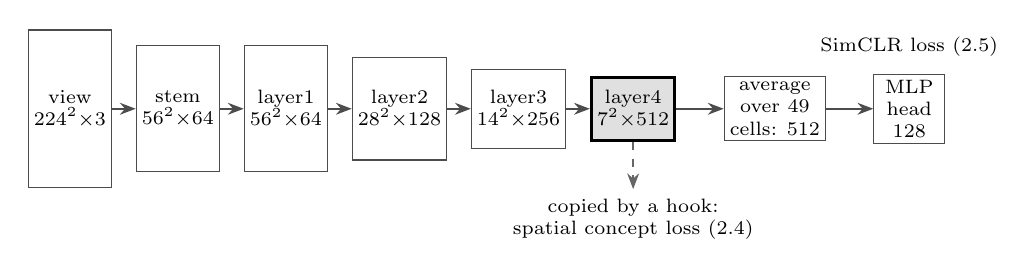
\begin{tikzpicture}[node distance=3mm,
 l/.style={draw=black!70,fill=white,minimum width=9mm,align=center,font=\scriptsize,inner sep=2pt}]
\node[l,minimum height=20mm] (in) {view\\$224^2{\times}3$};
\node[l,minimum height=16mm,right=of in] (c1) {stem\\$56^2{\times}64$};
\node[l,minimum height=16mm,right=of c1] (l1) {layer1\\$56^2{\times}64$};
\node[l,minimum height=13mm,right=of l1] (l2) {layer2\\$28^2{\times}128$};
\node[l,minimum height=10mm,right=of l2] (l3) {layer3\\$14^2{\times}256$};
\node[l,minimum height=8mm,right=of l3,fill=black!12,draw=black,very thick] (l4) {layer4\\$7^2{\times}512$};
\node[l,minimum height=6mm,right=6mm of l4] (gap) {average\\over 49\\cells: 512};
\node[l,minimum height=6mm,right=6mm of gap] (head) {MLP\\head\\128};
\draw[arr] (in)--(c1); \draw[arr] (c1)--(l1); \draw[arr] (l1)--(l2); \draw[arr] (l2)--(l3); \draw[arr] (l3)--(l4);
\draw[arr] (l4)--(gap); \draw[arr] (gap)--(head);
\node[above=1mm of head,font=\scriptsize] {SimCLR loss (2.5)};
\node[below=6mm of l4,font=\scriptsize,align=center] (hook) {copied by a hook:\\spatial concept loss (2.4)};
\draw[darr] (l4.south)--(hook.north);
\end{tikzpicture}
\caption{The ResNet-18 student. The resolution halves five times: $224/2^5=7$.}
\label{fig:resnet}
\end{figure}

\precise The ResNet-18 \citep{he2016resnet} maps a view to $H\in\mathbb R^{512\times7\times7}$ at the output of
\texttt{layer4}. Global average pooling gives $h=\frac1{49}\sum_u H(u)\in\mathbb R^{512}$, the feature the probe will
read after training. An MLP head maps $h$ to $g\in\mathbb R^{128}$ for the SimCLR loss. A forward hook keeps a copy of
$H$ for the spatial loss.

\why Location $(r,c)$ of $H$ sits over the 32-pixel square $(r,c)$ of the view, so each of the 49 vectors can be
asked about its own part of the view. After averaging, a cat and a sofa in the same view become one vector; before
averaging they are still at different locations. Class activation maps rest on the same property of this last map
\citep{zhou2016cam}.

\paragraph{Two different ``$7\times7$'' grids.} CLIP's window in step 1.5 also has $7\times7$ patches, because
$224/32=7$. The student's $7\times7$ in this step has the same size for a different reason ($224/2^5=7$). The two
grids never meet directly: CLIP's grid is turned into the $14\times14$ map of the whole image and step 2.3 resamples
that map to the student's grid of each view.

\subsection{Step 2.3: cut the matching piece out of the concept map}
\plain Each view shows only a piece of the photo, maybe mirrored. Its ``answer sheet'' must show the same piece. So we
take the photo's colouring-book map, cut out the same rectangle that the crop cut out of the photo, shrink it to
$7\times7$ squares and mirror it if the view was mirrored. Now square $(r,c)$ of the answer sheet describes exactly
the part of the view that the student's cell $(r,c)$ looks at.

\begin{figure}[H]
\centering
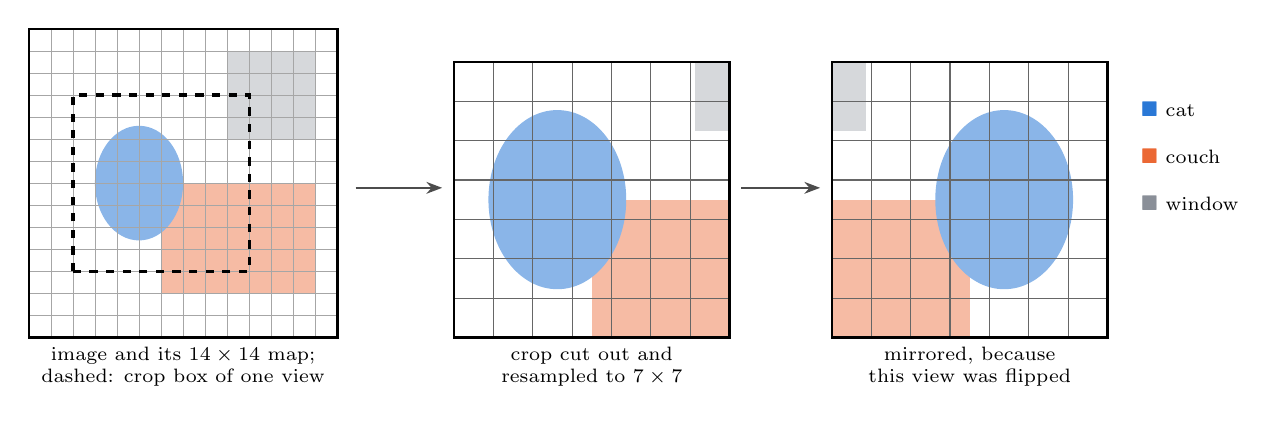
\begin{tikzpicture}
% full map
\begin{scope}[x=0.28cm,y=0.28cm]
\toyscene
\draw[black!35,very thin] (0,0) grid[step=1] (14,14);
\draw[thick] (0,0) rectangle (14,14);
\draw[very thick,dashed] (2,3) rectangle (10,11);
\node[font=\scriptsize,align=center,below] at (7,0) {image and its $14\times14$ map;\\dashed: crop box of one view};
\end{scope}
% cropped and resized
\begin{scope}[xshift=5.4cm]
\begin{scope}[x=0.4375cm,y=0.4375cm,shift={(-2,-3)}]
\clip (2,3) rectangle (10,11);
\toyscene
\end{scope}
\draw[black!60,thin] (0,0) grid[step=0.5cm] (3.5,3.5);
\draw[thick] (0,0) rectangle (3.5,3.5);
\node[font=\scriptsize,align=center,below] at (1.75,0) {crop cut out and\\resampled to $7\times7$};
\end{scope}
% flipped
\begin{scope}[xshift=10.2cm]
\begin{scope}[x=-0.4375cm,y=0.4375cm,shift={(-10,-3)}]
\clip (2,3) rectangle (10,11);
\toyscene
\end{scope}
\draw[black!60,thin] (0,0) grid[step=0.5cm] (3.5,3.5);
\draw[thick] (0,0) rectangle (3.5,3.5);
\node[font=\scriptsize,align=center,below] at (1.75,0) {mirrored, because\\this view was flipped};
\end{scope}
\draw[arr] (4.15,1.9) -- (5.25,1.9);
\draw[arr] (9.05,1.9) -- (10.05,1.9);
\node[font=\scriptsize,anchor=west] at (14.0,2.9) {\textcolor{catc}{$\blacksquare$} cat};
\node[font=\scriptsize,anchor=west] at (14.0,2.3) {\textcolor{couchc}{$\blacksquare$} couch};
\node[font=\scriptsize,anchor=west] at (14.0,1.7) {\textcolor{windowc}{$\blacksquare$} window};
\end{tikzpicture}
\caption{Warping the map onto one view (toy scene). Each of the $K$ channels of the map is cut and resampled in the
same way; the figure colours each cell by its winning factor.}
\label{fig:warp}
\end{figure}

\precise For a view with box (top $a$, left $b$, height $\eta$, width $\omega$, all as fractions of the image), the
box in map coordinates is $[14b,\,14(b+\omega)]\times[14a,\,14(a+\eta)]$. RoIAlign \citep{he2017maskrcnn} divides it into
$7\times7$ bins and averages $2\times2$ bilinear samples of $\tilde M_i$ inside each bin; a flipped view gets its target
mirrored along the width (\texttt{warp\_maps}). The result is $Y^{(v)}\in\mathbb R^{K\times7\times7}$, the target of
view $v$.

\why The crop box is stored as fractions of the original image and the map covers the whole image, so the box can be
placed on the map whatever the original size; resizing the image to $448\times448$ for the map does not change the
fractions. RoIAlign reads the map at exact fractional positions, so a crop that starts in the middle of a cell gets the
right values. A crop of 20\% area spans about $0.45\times14\approx6$ cells per side, so even the smallest crop has
real content for its $7\times7$ target.

\subsection{Step 2.4: the spatial concept loss}
This step is where the concepts enter training. It has four parts.

\paragraph{(a) Make 6,272 question--answer pairs per half.}
\plain Every one of the 49 cells of every view becomes one question: ``here are your 512 numbers for this cell;
which concepts are here?''. The answer is the matching cell of the answer sheet from step 2.3.

\precise Each location $u$ of view $v$ gives a row $r=H^{(v)}(u)/\lVert H^{(v)}(u)\rVert\in\mathbb R^{512}$ and a target
$y=Y^{(v)}(u)\in\mathbb R^{K}$. The 128 images of the batch are split into halves $A$ and $B$ of 64 images, both
views of an image always in the same half. Each half holds $64\times2\times49=6{,}272$ pairs $(r,y)$.

\begin{figure}[H]
\centering
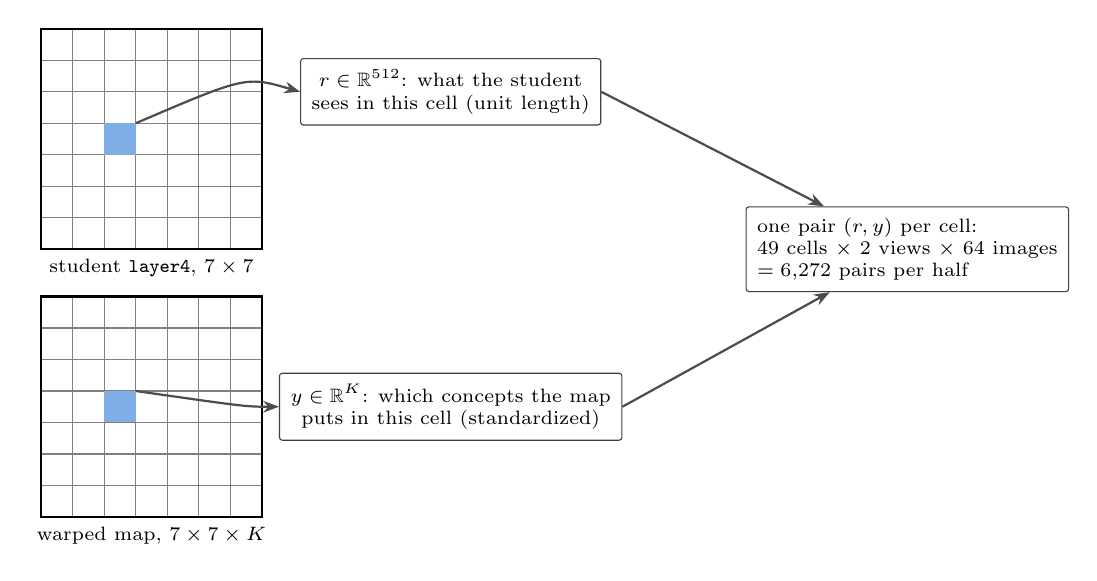
\begin{tikzpicture}
\begin{scope}
\draw[black!50] (0,0) grid[step=0.4cm] (2.8,2.8);
\draw[thick] (0,0) rectangle (2.8,2.8);
\fill[catc!60] (0.8,1.2) rectangle ++(0.4,0.4);
\node[font=\scriptsize,below] at (1.4,0) {student \texttt{layer4}, $7\times7$};
\end{scope}
\node[box,font=\scriptsize] (r) at (5.2,2.0) {$r\in\mathbb R^{512}$: what the student\\sees in this cell (unit length)};
\begin{scope}[yshift=-3.4cm]
\draw[black!50] (0,0) grid[step=0.4cm] (2.8,2.8);
\draw[thick] (0,0) rectangle (2.8,2.8);
\fill[catc!60] (0.8,1.2) rectangle ++(0.4,0.4);
\node[font=\scriptsize,below] at (1.4,0) {warped map, $7\times7\times K$};
\end{scope}
\node[box,font=\scriptsize] (y) at (5.2,-2.0) {$y\in\mathbb R^{K}$: which concepts the map\\puts in this cell (standardized)};
\draw[arr] (1.2,1.6) .. controls (2.6,2.2) .. (r.west);
\draw[arr] (1.2,-1.8) .. controls (2.6,-2.0) .. (y.west);
\node[box,font=\scriptsize,align=left] (pair) at (11.0,0) {one pair $(r,y)$ per cell:\\49 cells $\times$ 2 views $\times$ 64 images\\$=6{,}272$ pairs per half};
\draw[arr] (r.east) -- (pair);
\draw[arr] (y.east) -- (pair);
\end{tikzpicture}
\caption{The same cell of the student's feature map and of the warped map form one question--answer pair.}
\label{fig:pairs}
\end{figure}

\paragraph{(b) Learn a translation rule on half $A$.}
\plain On half $A$ we find the best simple rule that turns the student's 512 numbers into concept values. The rule is a
table $W$: for each concept, a direction in the student's feature space; the predicted value of ``cat'' in a cell is
how far the cell's vector points along the cat direction. The rule is found by a formula in one go, with no training.

\precise Weighted ridge regression, solved in closed form,
\begin{equation}
W_A=\big(\bar R_A^\top\Omega_A\bar R_A+\rho I\big)^{-1}\bar R_A^\top\Omega_A\,(Y_A-\bar y_A)\ \in\mathbb R^{512\times K},
\end{equation}
where $\bar R_A$ stacks the 6,272 rows of $A$ minus their weighted mean $\bar r_A$, $Y_A$ the targets, $\bar y_A$ their
weighted mean, $\Omega_A$ the per-row weights and $\rho=1$. The solve is one $512\times512$ linear system in float32.

\paragraph{(c) Test the rule on half $B$.}
\plain We use the rule from half $A$ to predict the concepts in every cell of half $B$ and measure how wrong it is. Then
we swap: a rule from $B$ is tested on $A$. The loss is the average mistake on the half the rule has not seen.

\precise
\begin{equation}
\hat Y_B=(R_B-\bar r_A)\,W_A+\bar y_A,\qquad
\mathcal L_{\text{spatial}}=\tfrac12\Big(\operatorname{err}(\hat Y_B,Y_B)+\operatorname{err}(\hat Y_A,Y_A)\Big),
\end{equation}
with $\operatorname{err}$ the weighted mean over views of $\frac1{49K}\lVert\hat Y_v-Y_v\rVert^2$
(\texttt{spatial\_cross\_fit\_loss}). Because the targets have variance 1, $1-\text{err}$ is the held-out explained
variance, logged during training.

\paragraph{(d) Push the student.}
\plain The rule itself is thrown away after the step. What we keep is the lesson for the student: ``change your 512
numbers so that next time a rule learned on some photos works better on other photos''.

\precise Gradients of $\mathcal L_{\text{spatial}}$ flow through the prediction and through the solve for $W_A$ into
$H$ and the ResNet weights \citep{bertinetto2019r2d2}. The ridge has no parameters of its own; it is solved again in
every step from the current features.

\begin{figure}[H]
\centering
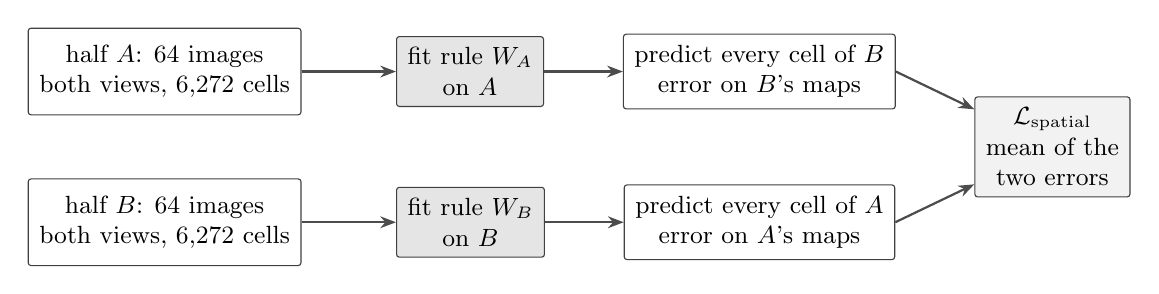
\begin{tikzpicture}[node distance=4mm]
\node[box,minimum width=26mm,minimum height=11mm] (A) {half $A$: 64 images\\both views, 6,272 cells};
\node[box,minimum width=26mm,minimum height=11mm,below=8mm of A] (B) {half $B$: 64 images\\both views, 6,272 cells};
\node[lbox,right=12mm of A] (fitA) {fit rule $W_A$\\on $A$};
\node[lbox,right=12mm of B] (fitB) {fit rule $W_B$\\on $B$};
\node[box,right=10mm of fitA] (predB) {predict every cell of $B$\\error on $B$'s maps};
\node[box,right=10mm of fitB] (predA) {predict every cell of $A$\\error on $A$'s maps};
\node[tbox,right=10mm of $(predB.east)!0.5!(predA.east)$] (loss) {$\mathcal L_{\text{spatial}}$\\mean of the\\two errors};
\draw[arr] (A)--(fitA); \draw[arr] (B)--(fitB);
\draw[arr] (fitA)--(predB); \draw[arr] (fitB)--(predA);
\draw[arr] (predB.east)--(loss); \draw[arr] (predA.east)--(loss);
\end{tikzpicture}
\caption{Cross-fitting: each rule is tested only on images it was not fitted on.}
\label{fig:crossfit}
\end{figure}

\why The cross-fit is the heart of the method and the lesson of the image-level experiments. Suppose the student
learned to recognise each photo individually (``this is photo 371'') and stored the answers of photo 371 somewhere in
its features. A rule fitted on half $A$ could then reproduce $A$'s answers, but it would be useless on half $B$, whose
photos it has never seen; memorising photos earns nothing. The only way to lower the loss is a \emph{shared} code:
cat-ness in the same direction in every photo, couch-ness in another direction, so that one rule works everywhere.
This is the sample splitting of double machine learning \citep{chernozhukov2018dml} applied to a training loss. With
a trained head in its place, the student fitted shuffled targets almost as well as real ones on MetaShift
\citep{zhang2017rethinking}.

The other choices of this step:
\begin{itemize}[leftmargin=*]
\item \textbf{Unit-length rows and an absolute ridge $\rho=1$.} If the student could shrink its features, it would
weaken the ridge and let the rule overfit. Unit rows fix the scale; $\rho=1$ keeps the $512\times512$ system well
conditioned \citep{hoerl1970ridge}. An earlier version without them produced NaN features.
\item \textbf{A linear rule.} The probe that evaluates the student after training is linear, so the concepts must be
\emph{linearly} readable from the features.
\item \textbf{Both views in one half.} Otherwise half $B$ would contain the other view of a photo in half $A$, and
recognising the photo would pay off again.
\item \textbf{6,272 rows against 512 dimensions.} Twelve times more rows than unknowns per concept: the fit is well
posed. A batch of 128 gives this ratio; the image-level version had only 128 rows per half.
\end{itemize}

\paragraph{The 20\% hold-out.} A fixed fifth of the training images (340 on MetaShift) gets weight $\omega=0$ in
$\Omega$: their cells neither shape any rule nor count in the error. SimCLR still trains on them. After training they
show whether the student's concepts carry over to images that never entered the concept loss. The arm with this
hold-out also scored higher than the arm without it, so it stayed in the main configuration.

\subsection{Step 2.5: the SimCLR loss, unchanged}
\plain Among the 256 views in the batch, every view has exactly one partner: the other version of the same photo.
The student must make the summaries of partners similar and the summaries of all other views different. It is a
game of ``find your twin among 255 strangers''.

\begin{figure}[H]
\centering
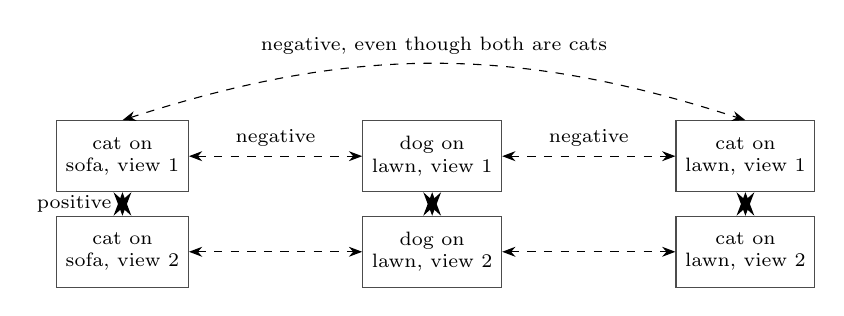
\begin{tikzpicture}[node distance=3mm,
 v/.style={draw=black!70,minimum width=13mm,minimum height=9mm,font=\scriptsize,align=center}]
\node[v] (a1) {cat on\\sofa, view 1};
\node[v,below=of a1] (a2) {cat on\\sofa, view 2};
\node[v,right=22mm of a1] (b1) {dog on\\lawn, view 1};
\node[v,below=of b1] (b2) {dog on\\lawn, view 2};
\node[v,right=22mm of b1] (c1) {cat on\\lawn, view 1};
\node[v,below=of c1] (c2) {cat on\\lawn, view 2};
\draw[very thick,{Stealth}-{Stealth}] (a1)--(a2) node[midway,left,font=\scriptsize]{positive};
\draw[very thick,{Stealth}-{Stealth}] (b1)--(b2);
\draw[very thick,{Stealth}-{Stealth}] (c1)--(c2);
\draw[dashed,{Stealth}-{Stealth}] (a1)--(b1) node[midway,above,font=\scriptsize]{negative};
\draw[dashed,{Stealth}-{Stealth}] (b1)--(c1) node[midway,above,font=\scriptsize]{negative};
\draw[dashed,{Stealth}-{Stealth}] (a2)--(b2);
\draw[dashed,{Stealth}-{Stealth}] (b2)--(c2);
\draw[dashed,{Stealth}-{Stealth}] (a1.north) to[bend left=18] node[above,font=\scriptsize]{negative, even though both are cats} (c1.north);
\end{tikzpicture}
\caption{SimCLR pairs. Each view's positive is the other view of its own image; all 254 other views are negatives,
including other cats.}
\label{fig:simclr}
\end{figure}

\precise With $g_v\in\mathbb R^{128}$ the normalized projection of view $v$, $v^+$ its partner and $\tau=0.05$, the
NT-Xent (InfoNCE) loss \citep{oord2018cpc,chen2020simclr} is
\begin{equation}
\mathcal L_{\text{SimCLR}}=-\frac1{2B}\sum_{v=1}^{2B}\log
\frac{\exp(g_v^\top g_{v^+}/\tau)}{\sum_{w\ne v}\exp(g_v^\top g_w/\tau)} .
\end{equation}

\why SimCLR is the self-supervised method all our comparisons share. It needs no labels, but it rewards any feature
that tells photos apart, the sofa as much as the cat; on a dataset where sofa and cat come together, it has no reason
to separate them. The spatial loss of step 2.4 adds that reason.

\subsection{Step 2.6: add the two losses and update}
\plain The final score is the SimCLR score plus the concept score times a weight. For the first ten epochs the weight
is zero, so the student first learns ordinary SimCLR; over the next ten epochs the weight grows to 5 and stays there.

\precise
\begin{equation}
\mathcal L=\mathcal L_{\text{SimCLR}}+\lambda(t)\,\mathcal L_{\text{spatial}},\qquad
\lambda(t)=\begin{cases}0,& t\le10,\\ 5\,(t-10)/10,& 10<t<20,\\ 5,& t\ge20,\end{cases}
\end{equation}
with $t$ the epoch. SGD (learning rate 0.01, decayed by 0.1 at epochs 350, 400 and 450, weight decay $10^{-4}$) updates
the ResNet and the MLP head; float16 autocast runs the network, float32 the ridge solve.

\begin{figure}[H]
\centering
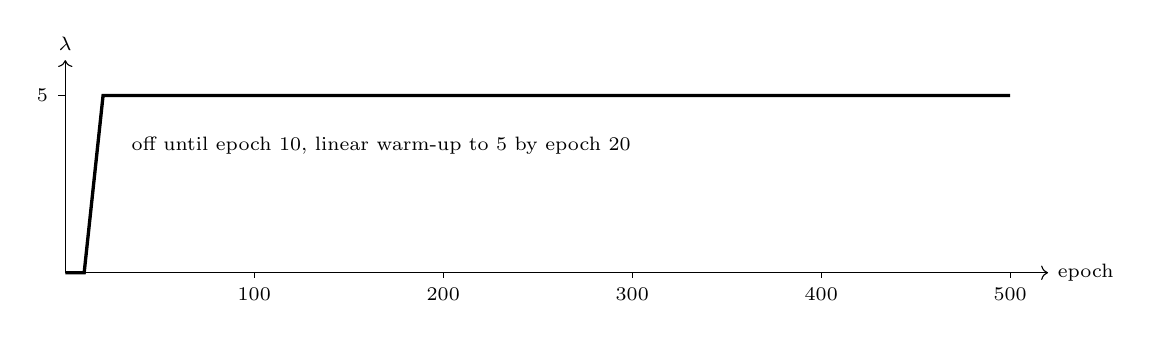
\begin{tikzpicture}[x=0.024cm,y=0.45cm]
\draw[->] (0,0) -- (520,0) node[right,font=\scriptsize]{epoch};
\draw[->] (0,0) -- (0,6) node[above,font=\scriptsize]{$\lambda$};
\draw[very thick] (0,0) -- (10,0) -- (20,5) -- (500,5);
\foreach \x in {100,200,300,400,500} \draw (\x,0) -- ++(0,-0.15) node[below,font=\scriptsize]{\x};
\draw (0,5) -- ++(-4,0) node[left,font=\scriptsize]{5};
\node[font=\scriptsize,anchor=west] at (30,3.6) {off until epoch 10, linear warm-up to 5 by epoch 20};
\end{tikzpicture}
\caption{Weight of the spatial concept loss over training.}
\end{figure}

\why SimCLR first forms usable features; a concept loss on random features at epoch 0 would mostly add noise. The
weight 5 came from a grid of 1, 3, 5 and 10; weight 10 added nothing.

%=====================================================================
\section{Stage 3: evaluation}
%=====================================================================
\plain After training we keep only the student. For each photo it gives one summary of 512 numbers. A very simple
classifier (a line through the space of summaries) learns cat versus dog from a small set with equally many photos of
each kind: cats indoors, cats outdoors, dogs indoors, dogs outdoors. We then check its accuracy on each of the four
kinds separately and report the worst one.

\precise Every 25 epochs a logistic regression (L2 coefficient 0.001) is fitted on the pooled 512-d features of a
group-balanced subset of the training split (400 images on MetaShift) and evaluated on the validation split; the
reported value is the mean of the last four probes (epochs 425 to 500). Labels appear only here.

\why A balanced linear probe recovers the class whenever the representation holds the class and the spurious attribute
in separate directions \citep{kirichenko2023dfr}. The spatial loss aims for exactly that: a cat direction that the
probe can use on cats outdoors.

%=====================================================================
\section{Why this should help and what it achieves}
%=====================================================================
\paragraph{The argument.} At the level of whole photos, ``cat'' and ``sofa'' arrive together on 88\% of MetaShift's
training images; a student that only sees whole photos can satisfy every whole-photo target with one fused
``cat-and-sofa'' feature. At the level of cells, the cat and the sofa sit in different cells of \emph{every} photo. A
single rule that predicts ``cat here, sofa there'' for photos it has not seen requires the student to code cat-ness and
sofa-ness separately, in the same way across photos. The balanced probe can then pick the cat direction.

\paragraph{What it achieves.} Validation WGA rises over SimCLR by 6.1 points on Waterbirds (46.7 to 52.8), 6.8 on
MetaShift (44.3 to 51.1) and 22.5 on Spur-CIFAR10 (15.6 to 38.1). The same loss with another photo's maps (shuffled
control) stays at the SimCLR level, so the gain comes from each photo's own maps. On the 20\% held-out images the student
predicts the concepts as well as on the images inside the loss: it learned shared concepts.

\paragraph{Where it stops.} A cell of the student's $7\times7$ map is computed from a large part of the view
\citep{luo2016erf}, so the cell over the cat also sees the sofa. The cheapest way to predict ``cat here'' still uses the
sofa, which is right 88\% of the time. The audit confirms it: the student's cat factor scores 0.47 on unseen cats indoors
and 0.07 on unseen cats outdoors, against 0.92 and 0.88 for CLIP. SCD makes the cat feature stronger; it does not yet
free it from the sofa. Section~8 of the main report describes the attempts to go further.

%=====================================================================
\section{The same algorithm as pseudocode}
%=====================================================================
\begin{verbatim}
# ---------- Stage 1: once per dataset (frozen CLIP, no labels) ----------
z      = clip.encode_image(images_224)               # N x 512
codes  = splice(z, vocabulary, l1=0.25)              # N x 10000, ~9 non-zero
factors, d = meaning_grouping(codes, text_emb)       # K factors, d: K x 512
for image in dataset:
    big   = resize(image, 448, 448)
    score = zeros(K, 28, 28); count = zeros(28, 28)
    for top in (0, 112, 224):
        for left in (0, 112, 224):
            p = clearclip_patches(big[top:top+224, left:left+224])  # 7x7x512
            s = p @ d.T                                              # 7x7xK
            score += s spread to 2x2 cells; count += 1
    maps[image] = softmax(avgpool(score / count, 14) / 0.01, dim=K)  # K x14x14
maps = standardize_per_factor(maps)

# ---------- Stage 2: every training step ----------
for images in batches_of_128:
    v1, box1 = augment(images); v2, box2 = augment(images)  # crop+flip recorded
    H = resnet.layer4(cat(v1, v2))           # 256 x 512 x 7 x 7  (hook)
    g = mlp(avgpool(H))                       # 256 x 128
    loss_ssl = nt_xent(g, temperature=0.05)
    Y = roi_align(maps[images], cat(box1, box2), 7x7)  # then flip flipped views
    R = normalize(H per location)             # rows of 512
    A, B = halves of the 128 images (both views together)
    W_A = ridge(R[A], Y[A], weights, rho=1); W_B = ridge(R[B], Y[B], ...)
    loss_spatial = (mse(R[B] @ W_A, Y[B]) + mse(R[A] @ W_B, Y[A])) / 2
    loss = loss_ssl + lambda(epoch) * loss_spatial
    loss.backward(); sgd.step()   # grads pass through the solve

# ---------- Stage 3: evaluation ----------
probe = logistic_regression(avgpool(resnet(balanced_images)), labels)
report worst_group_accuracy(probe, validation)
\end{verbatim}

%=====================================================================
\section{Glossary}
%=====================================================================
\begin{table}[H]
\centering
\small
\begin{tabularx}{\linewidth}{l X}
\toprule
Term & Meaning \\
\midrule
View & One randomly edited copy of a photo (crop, flip, colour); SimCLR uses two per photo \\
Crop box & The rectangle a view was cut from, stored as fractions of the photo \\
Flip & Left--right mirroring, applied to half of the views \\
Positive / negative & In SimCLR: the other view of the same photo / every view of another photo \\
Patch & A $32\times32$-pixel square that CLIP's vision transformer turns into one vector \\
ClearCLIP & CLIP with a modified last block whose patch vectors match text locally \\
Concept factor & A group of synonyms (\{cat, kitten, kitty\}) with one text direction \\
Concept map & For one photo: $14\times14$ cells, each with shares of the $K$ factors summing to 1 \\
Warping & Cutting a view's crop box out of the map and resampling it to $7\times7$ (RoIAlign) \\
Feature map & The student's \texttt{layer4} output, $7\times7$ cells of 512 numbers \\
Cross-fit & Fit the rule on one half of the batch, measure its error on the other half \\
Ridge & Least-squares fit of a linear rule with a penalty $\rho$ that keeps it stable \\
Hold-out & 20\% of photos that never enter the concept loss, used to check generalization \\
WGA & Worst-group accuracy: accuracy on the hardest of the four (class, background) groups \\
\bottomrule
\end{tabularx}
\end{table}

\begingroup
\small
\setlength{\bibsep}{3pt plus 1pt}
\begin{thebibliography}{99}
\bibitem[Bertinetto et~al.(2019)]{bertinetto2019r2d2}
L.~Bertinetto, J.~F.~Henriques, P.~H.~S.~Torr and A.~Vedaldi. Meta-learning with Differentiable Closed-Form Solvers.
\emph{ICLR}, 2019. \url{https://arxiv.org/abs/1805.08136}.
\bibitem[Bhalla et~al.(2024)]{bhalla2024splice}
U.~Bhalla, A.~Oesterling, S.~Srinivas, F.~P.~Calmon and H.~Lakkaraju. Interpreting CLIP with Sparse Linear Concept
Embeddings (SpLiCE). \emph{NeurIPS}, 2024. \url{https://arxiv.org/abs/2402.10376}.
\bibitem[Chen et~al.(2020)]{chen2020simclr}
T.~Chen, S.~Kornblith, M.~Norouzi and G.~Hinton. A Simple Framework for Contrastive Learning of Visual Representations.
\emph{ICML}, 2020. \url{https://arxiv.org/abs/2002.05709}.
\bibitem[Chernozhukov et~al.(2018)]{chernozhukov2018dml}
V.~Chernozhukov et~al. Double/Debiased Machine Learning for Treatment and Structural Parameters. \emph{The Econometrics
Journal}, 21(1), 2018. \url{https://arxiv.org/abs/1608.00060}.
\bibitem[Darcet et~al.(2024)]{darcet2024registers}
T.~Darcet, M.~Oquab, J.~Mairal and P.~Bojanowski. Vision Transformers Need Registers. \emph{ICLR}, 2024.
\url{https://arxiv.org/abs/2309.16588}.
\bibitem[He et~al.(2016)]{he2016resnet}
K.~He, X.~Zhang, S.~Ren and J.~Sun. Deep Residual Learning for Image Recognition. \emph{CVPR}, 2016.
\url{https://arxiv.org/abs/1512.03385}.
\bibitem[He et~al.(2017)]{he2017maskrcnn}
K.~He, G.~Gkioxari, P.~Doll\'ar and R.~Girshick. Mask R-CNN. \emph{ICCV}, 2017. \url{https://arxiv.org/abs/1703.06870}.
\bibitem[Hoerl and Kennard(1970)]{hoerl1970ridge}
A.~E.~Hoerl and R.~W.~Kennard. Ridge Regression: Biased Estimation for Nonorthogonal Problems. \emph{Technometrics},
12(1), 1970.
\bibitem[Kirichenko et~al.(2023)]{kirichenko2023dfr}
P.~Kirichenko, P.~Izmailov and A.~G.~Wilson. Last Layer Re-Training is Sufficient for Robustness to Spurious
Correlations. \emph{ICLR}, 2023. \url{https://arxiv.org/abs/2204.02937}.
\bibitem[Lan et~al.(2024)]{lan2024clearclip}
M.~Lan et~al. ClearCLIP: Decomposing CLIP Representations for Dense Vision-Language Inference. \emph{ECCV}, 2024.
\url{https://arxiv.org/abs/2407.12442}.
\bibitem[Luo et~al.(2016)]{luo2016erf}
W.~Luo, Y.~Li, R.~Urtasun and R.~Zemel. Understanding the Effective Receptive Field in Deep Convolutional Neural
Networks. \emph{NeurIPS}, 2016. \url{https://arxiv.org/abs/1701.04128}.
\bibitem[van den Oord et~al.(2018)]{oord2018cpc}
A.~van den Oord, Y.~Li and O.~Vinyals. Representation Learning with Contrastive Predictive Coding. \emph{arXiv:1807.03748},
2018. \url{https://arxiv.org/abs/1807.03748}.
\bibitem[Radford et~al.(2021)]{radford2021clip}
A.~Radford et~al. Learning Transferable Visual Models From Natural Language Supervision. \emph{ICML}, 2021.
\url{https://arxiv.org/abs/2103.00020}.
\bibitem[Wang et~al.(2024)]{wang2024sclip}
F.~Wang, J.~Mei and A.~Yuille. SCLIP: Rethinking Self-Attention for Dense Vision-Language Inference. \emph{ECCV}, 2024.
\url{https://arxiv.org/abs/2312.01597}.
\bibitem[Zhang et~al.(2017)]{zhang2017rethinking}
C.~Zhang, S.~Bengio, M.~Hardt, B.~Recht and O.~Vinyals. Understanding Deep Learning Requires Rethinking Generalization.
\emph{ICLR}, 2017. \url{https://arxiv.org/abs/1611.03530}.
\bibitem[Zhou et~al.(2016)]{zhou2016cam}
B.~Zhou, A.~Khosla, A.~Lapedriza, A.~Oliva and A.~Torralba. Learning Deep Features for Discriminative Localization.
\emph{CVPR}, 2016. \url{https://arxiv.org/abs/1512.04150}.
\bibitem[Zhou et~al.(2022)]{zhou2022maskclip}
C.~Zhou, C.~C.~Loy and B.~Dai. Extract Free Dense Labels from CLIP. \emph{ECCV}, 2022.
\url{https://arxiv.org/abs/2112.01071}.
\end{thebibliography}
\endgroup

\end{document}
